\chapter{Análisis topológico de trayectorias en alta y baja dimensión} \label{chp:desarrollo}

El desarrollo de este proyecto se puede dividir principalmente en 4 secciones, selección y preparación de los datos a utilizar durante el desarrollo del proyecto, en segundo lugar la elección de la metodología de análisis a seguir durante el desarrollo del mismo, y las herramientas computacionales y de software que se emplearon para realizar dicho análisis. En tercer lugar, el diseño e implementación de la solución, explicando las decisiones tomadas durante el diseño de la misma, y finalmente, estudio de la solución y pruebas realizadas para comprobar la eficacia de la misma.

\section{Modelización de los datos}

\subsection{Selección de los datos}
A lo hora de seleccionar los datasets de trayectorias utilizados para el desarrollo delo trabajo, se tuvieron en cuenta varios factores. El primero de ellos fue las licencias de uso de los mismos, reduciendo la búsqueda a datasets con licencia CC0, es decir, aquellos de datos que fueran denominados de dominio público. En segundo lugar, se tuvieron en cuenta los criterios estándar para la calidad del dato, es decir, se tuvo en la precisión (falta de errores), la integridad (ausencia de columnas vacías o datos inexistentes), consistencia y unicidad de los mismos. Asimismo, se tuvo en cuenta el formato de los datasets, evaluando la compatibilidad de estos con las librerías que se usarían durante el desarrollo del proyecto, y las posibilidad de deformaciones en caso de haber la necesidad de oficiar los mismos para adaptarlos a las herramientas. Finalmente, se evaluó el contenido de los mismos, analizando minuciosamente las posibilidades que la trayectorias contenidas en los mismos aportaban de cara a su manipulación y análisis durante el desarrollo del proceso.


Atendido a los criterios anteriormente mencionados, finalmente se tomó la decisión de usar el dataset GeoLife GPS Trajectories \cite{geolife_datos} . Esto se debe a la gran variedad de datos que nos presenta el dataset, teniendo trayectorias pequeños, fácilmente manejables sin gastar en exceso en recursos computacionales, como trayectorias más extensas, con más posibilidad de obtener resultados más vistosos de cara a analizar su topología, así como la posibilidad de realizar análisis con un conjunto de estas trayectorias simultáneamente. 

Estas trayectorias se encuentran en formato .plt, ofrenciéndonos la oportunidad de utilizar las herramientas de análisis sin realizar ningún tipo de modificación sobre los mismos. En lo que al contenido se refiere, estos datos contienen datos de trayectorias GPS de 178 usuarios durante un período de cuatro años, siendo cada trayectoria representada por una secuencia de puntos marcados en el tiempo, conteniendo aparte de su información temporal, información sobre la latitud, longitud y altitud en cada uno de estos instantes temporales, pudieron realizar en primer instante análisis sobre las 3 dimensiones del espacio, pudiendo escalarlo añadiéndole lag o desfases usando funciones internas de la libraría en caso de desear realizar análisis más complejos sobre el conjunto de datos, siendo este obligado en el ámbito de las dependencias temporales y espaciales de las trayectorias. \cite{geolife1} \cite{geolife2} \cite{geolife3} 

\subsection{Preparación de los datos}

De cara a la preparación de los datos a utilizar, se realizo un estudio del contenido de los mismos durante la selección, como se mencionó en la sección anterior, para garantizar la integridad y completitud de los mismos. Posteriormente, se revisó más en detalles el formato de los campos y los valores de los mismos para preparar código para la lectura y la composición de un dataframe de \textit{Pandas} (librería de Python, una de las herramientas que se usará durante el desarrollo) de cara a generar el array de puntos necesaria para el uso de la funciones de la librería \textit{giotto-tda} \cite{Giotto-tda}. Este array de la nube puntos se trata de un \textit{ndarray}, de la librería \textit{NumPy}. Estos array se caracterizan por ser estructuras n-dimensionales, homogéneas y de tamaño fijo, construyéndose a partir del dataframe generado, seleccionando los valores de latitud, longitud y altitud, haciendo uso de la función \textit{.values()} propia de los dataframe de \textit{Pandas}.

\section{Metodología y herramientas para el análisis}

\subsection{Metodología de desarrollo}
En lo que a la metodología se refiere, se ha seguido un enfoque iterativo-exploratorio. En primer lugar, se realizó una etapa de preprocesamiento de los datos, que consistía en la lectura de trayectorias desde diferentes fuentes (\texttt{.plt}, \texttt{LINESTRING}, etc.), su transformación a nubes de puntos uniformes en dimensión y formato, y su normalización o reducción si fuera necesario. A continuación, se aplican las técnicas de análisis topológico, comenzando con el cálculo de diagramas de persistencia mediante filtraciones de Vietoris–Rips y la computación de medidas asociadas como la entropía de persistencia.

Posteriormente, se integró la herramienta Mapper, configurando un pipeline con funciones de filtrado (como proyecciones PCA), coberturas cúbicas e implementaciones de clustering como \texttt{DBSCAN}. Finalmente, se generaron grafos para facilitar la interpretación de la estructura topológica de las trayectorias a analizar.

Este enfoque ha permitido estudiar una variedad de configuraciones relativas al análisis, adaptándose al tamaño y características de la trayectoria o conjunto de trayectorias analizado en el momento, y facilitando la extracción de patrones generales y particularidades topológicas del movimiento en diferentes contextos.

\subsection{Herramientas utilizadas}

Como se mencionó anteriormente en el capítulo de Estado del Arte, existen una gran variedad de herramientas computacionales para la realización de análisis topológico de datos, permitiendo al usuario desarrollar con libertad en una variedad de entornos y lenguajes de programación las tareas de análisis que él desee. Nos hemos decidido por usar el lenguaje \textbf{Python}, debido a su amplia adopción en la comunidad científica, su sintaxis sencilla  y su gran oferta de bibliotecas para análisis de datos, visualización y aprendizaje automático. También ha ayudado a tomar esta decisión la familiaridad y experiencia con el uso de este lenguaje, y las facilidades que este da a la hora de ejecutar desde varias máquinas o entornos distintos, habiendo ejecutado las distintas implementaciones realizadas tanto en local como en entornos como \textbf{Google Colab}, para aprovechar los recursos extra que pudieran aportar de cara a agilizar los tiempos de ejecución de los procesos propios del análisis. 


La elección de Python como lenguaje para basar nuestro desarrollo nos da acceso a una amplia variedad de librerías que nos ayudarán en nuestro estudio, entre las cuáles cabe destacar las siguientes:

\begin{itemize}
    \item \textbf{NumPy} y \textbf{Pandas}: utilizadas para el tratamiento de datos y la conversión de trayectorias en arrays o dataframes.
    \item \textbf{Matplotlib} y \textbf{Seaborn}: utilizadas para la visualización de trayectorias, resultados intermedios, representaciones PCA y diagramas de persistencia.
    \item \textbf{Scikit-learn}: empleada para tareas de preprocesamiento (como la reducción de trayectorias mediante \texttt{KMeans}) y para clustering dentro del algoritmo Mapper.
    \item \textbf{Giotto-TDA} \cite{Giotto-tda}: una biblioteca especializada en análisis topológico de datos, desarrollada en Python sobre interfaces en C++, que ofrece implementaciones optimizadas para el cálculo de homología persistente y la construcción del grafo Mapper, entre otras funcionalidades.
\end{itemize}

\section{Diseño e implementación de soluciones con TDA}

Durante el desarrollo del trabajo se hizo uso de una serie de scripts de \textbf{Python}  para realizar análisis sobre una sola trayectoria del dataset Geolife y un conjunto de trayectorias del mismo, con herramientas TDA, y un script aplicando métodos no TDA como PCA, clustering tradicional y análisis t-SNE. Adicionalmente se añadió desplazamiento a los datos de las trayectorias para generar más diversidad al análisis, al darnos una visión adicional de las características topológicas de los datos.

\subsection{Carga de Trayectorias}
Para poder realizar cualquiera de estos análisis es fundamental realizar una correcta lectura y transformación de los datos de las trayectorias. Haciendo uso de la función \textit{read\_csv} de \textit{Pandas}, y la librería \textit{os}, se realiza una lectura del archivo o carpeta dependiendo del análisis que se desea realizar, generando un dataframe, y usando funciones de Pandas se eliminan los valores nulos en caso de haberlos, y se genera un dataframe de Pandas que contiene los valores de latitud, longitud y altitud de las trajectorias. Se establecieron también criterios para la toma de trayectorias, estableciendo como 50 el número mínimo de puntos que debe poseer el dataset para tenerlo en cuenta. Finalmente no hizo falta realizar ninguna tarea de limpieza ni transformación adicional, al poseer los datos escogidos una muy buena calidad en términos de lectura.

\subsection{Visualización de Nube de Puntos}
Después de la correcta lectura de los datos, se utiliza la función \textit{plot\_point\_cloud } para realizar una representación y visualización en tres dimensiones de la nube de puntos. Esta visualización nos permite obtener una idea preliminar de la distribución que siguen las trayectorias objeto del análisis. Cada trayectoria es representada como una secuencia de coordenadas geográficas, transformadas en puntos en tres dimensiones. En la figura \ref{fig:nube_puntos} se adjunta la nube de puntos generada por un conjunto de 110 trayectorias consecutivas, permitiéndonos observar la evolución de los recorridos y las estructuras topológicas que se van a analizar posteriormente. 

\begin{figure}[h]
    \centering
    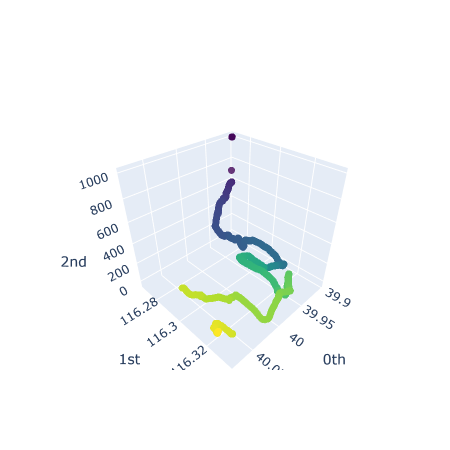
\includegraphics[scale=1]{images/Nube_Puntos.png}
    \caption{Visualización de la Nube de Puntos de las trayectorias de Geolife}
    \label{fig:nube_puntos}
\end{figure}


\vspace{5cm}

\subsection{Cálculo de Homologías Persistentes}

Una vez visualizados los datos, se procede a realizar un análisis utilizando la técnica de homologías persistentes, uno de los pilares fundamentales del análisis topológico de datos. Para la presente implementación, se decidió hacer uso de este método para el cálculo de homologías persistentes de complejos de \textit{Vietoris-Rips}, permitiéndonos extraer información clave sobre las características topológicas de los datos a lo largo de diferentes escalas. Esta implementación se realizó utilizando el módulo \textit{VietorisRipsPersistence} de la librería \textit{giotto-tda}, especificando como argumentos las dimensionales de homología que son de interées en el análisis, siendo en el ejemplo que se muestra en la Figura \ref{fig:pers_una} tres:

\begin{figure}[h]
    \centering
    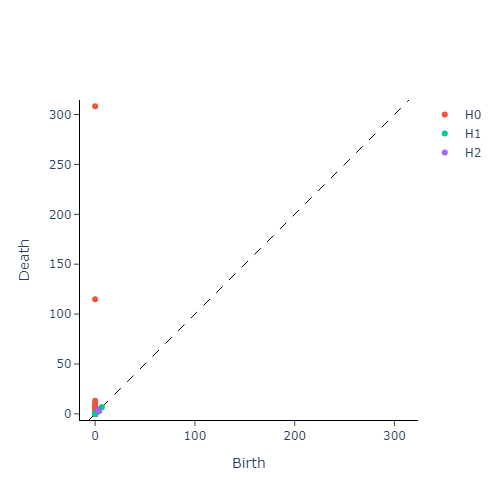
\includegraphics[scale=0.7]{images/persistencia.png}
    \caption{Diagrama de Persistencia de un Conjunto de trayectorias}
    \label{fig:pers}
\end{figure}

Estas tres dimensiones nos permiten observar diferentes estructuras topológicas:

\begin{enumerate}
    \item HO: Nos permite identificar las componentes conexas de la nube de puntos
    \item H1: Nos indica los ciclos presentes en el conjunto de los datos
    \item H2: Nos permite observar las cavidades, o huecos tridimensionales presentes en la estructura
\end{enumerate}

\vspace{2cm}
A la hora de realizar las ejecuciones de esta función, al usar volúmenes de datos de gran dimensiones, los tiempos de ejecución en la misma eran bastantes elevados, con un alto coste computacional, por tanto, se hizo usó de la integración de la librería \textit{giotto-tda} con paralelismo \textit{multi-thread} para agilizar estos procesos de cálculo y generación de gráficas, mejorando los tiempos de ejecución en alrededor de un 200\% usando 15 hilos ejecutando en una sola máquina. 

\begin{figure}[h]
    \centering
    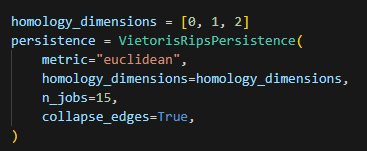
\includegraphics[scale=0.7]{images/codigo_persistencia.png}
    \caption{Definición del objeto VietorisRipsPersistence}
    \label{fig:codigo}
\end{figure}

Una vez hemos definido el objeto \textit{persistence} y realizados los cálculos, se procede a la representación gráfica del diagrama de persistencia, veáse Figura~\ref{fig:pers} . Esta representación se genera haciendo las transformaciones necesarias al objetivo persistencia generando mediante el uso de la función \textit{.fit\_transform}, generando así un objeto para mandar de argumento a la función \textit{plot\_diagram} para generar el diagrama mencionado anteriormente.

\subsection{Extracción de Descriptores con Mapper}

Llegados a este punto, habiendo realizado ya la visualización de los datos y el cálculo de las homologías persistentes, precedemos a la preparación de un pipeline de Mapper, y la representación en forma de grafo de este haciendo uso de las funciones de la librería \textit{giotto-tda}. En primera instancia, es importante dar una breve explicación de en que consiste el algoritmo: "\ Un conjunto de datos $S$, con los siguientes hiperparámetros, tiene asociado el complejo simplicial de Mapper:

\begin{itemize}
    \item Un algoritmo de clusterización y un conjunto de $n$ clústers.
    \item Una función filtro que capture variables latentes a un espacio de dimensión $K$.
    \item Una cubierta abierta de nuestro espacio de variables latentes.
    \item Para cada abierto $U$ del espacio latente y cada $i \leq K$, construimos un conjunto de puntos en $S$ determinado por el $i$-ésimo clúster de la imagen inversa de $U$, es decir, todos los elementos de la base de datos que bajo $f$ van a dar a $U$.
\end{itemize}

La familia de todos los subconjuntos $S(U,i)$ de la base de datos determinada por todas las parejas $(U,i)$ serán los puntos de nuestro complejo simplicial de Mapper. Las caras de este complejo simplicial están determinadas por los subconjuntos que contengan registros de nuestro dataset en común."\   \cite{bourbaki_mapper}

\vspace{5cm}

Teniendo esto en cuenta, procedemos al diseño y configuración del pipeline. Este proceso se compone de los siguientes cuatros pasos:

\begin{itemize}
    \item \textbf{Cartografía} En primer lugar, cartografiamos $D$ a un espacio de menor dimensión usando una función de filtrado de tipo $f: R^n -> R^m$. Se puede elegir de una variedad de funciones para realizar esta tarea, en nuestro análisis decimos hacer uso de una proyección, al darnos la opción la opción de realizar distintos análisis con cambios mínimos en los parámetros del análisis. Todo esto se consigue haciendo uso de la función \textit{FilterFunctionName} de la librería \textit{giotto-tda}, que contiene una gran de variedad de funciones de filtrado, dando libertad al usuario para ajustar el análisis que desea realizar a las características del problema o datos a tratar.  
    \item \textbf{Filtrado} Una vez realizado la proyección, se procede al filtrado de valores de tipo ${\cal U } = (U_i)_ {i\in I}$, para generar un recubrimiento de un conjunto de intervalos que se solapan, con una longitud constante.En esta implementación, se hace uso de un recubrimiento de tipo \texttt{CubicalCover} con \texttt{n\_intervals = 10} y \texttt{overlap\_frac = 0.4}, lo que significa que el espacio filtrado se divide en 10 intervalos por dimensión, cada uno con un solapamiento del 40\%. Esta superposición es esencial para capturar estructuras conectadas en regiones vecinas y evitar una fragmentación excesiva del espacio.
    \item \textbf{Clusterización} Para cada conjunto preimagen $f^{-1}(U_i)$ asociado a cada intervalo del recubrimiento, se aplica un algoritmo de agrupamiento con el objetivo de identificar componentes conexas. En nuestro caso, se emplea el algoritmo \texttt{DBSCAN} (Density-Based Spatial Clustering of Applications with Noise), que tiene la ventaja de no requerir especificar el número de clusters y es robusto frente al ruido y las formas arbitrarias de los datos. Esto lo convierte en una opción adecuada para trayectorias geográficas, donde pueden existir regiones de alta densidad intercaladas con trayectorias dispersas o inusuales.

    \item \textbf{Construcción del grafo} Finalmente, se construye un grafo Mapper, en el cual cada nodo representa un cluster obtenido en algún intervalo, y se crea una arista entre dos nodos si comparten al menos un punto de datos (es decir, si sus conjuntos de puntos tienen intersección no vacía). Este grafo sintetiza la estructura topológica del conjunto de datos original, revelando la conectividad global, la presencia de ciclos o componentes separados, y sirve como herramienta de exploración visual y estructural. 
\end{itemize}

Para la visualización del grafo Mapper resultante del proceso descrito anteriormente, se utiliza la función \texttt{plot\_static\_mapper\_graph} de \texttt{giotto-tda}, que genera una representación estática del grafo que puede ser interpretada fácilmente en el contexto de las trayectorias geoespaciales. Adicionalmente, se hace uso nuevamente de la integración de la librería con paralelismo \textit{multi-thread}, para agilizar la ejecución de la creación de los pipelines de Mapper.

A continuación, se puede ver el resultado de ejecutar este proceso, con un pipeline definido de la siguiente manera: una función de proyección sobre los 3 ejes cartesianos, con un recubrimiento cúbico, y un solapamiento de un 30\%:

\begin{figure}
    \centering
    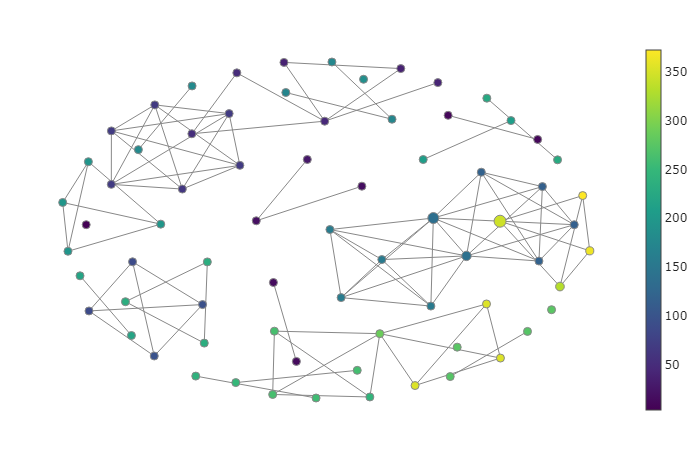
\includegraphics[scale=0.7]{images/mapper.png}
    \caption{Grafo de Mapper generado a partir de una trayectoria del Dataset}
    \label{fig:grafo_mapper}
\end{figure}


\vspace{20cm}
Adicionalmente, para algunas trayectorias en concreto se genero la matriz de distancias haciendo uso de la librería dedicada para Machine Learning de Python, \textit{sklearn}, mas concretamente la funcion \textit{pairwise\_distances}, utilizando la métrica euclidiana, y representando esta gráfica en formato mapa de calor, para visualizar de mejor manera las distancias entre las componentes de la trayectoria.

\subsection{Análisis y comparación con PCA}

Para complementar el análisis topológico y obtener una representación reducida de los datos de trayectoria, se ha empleado la técnica de Análisis de Componentes Principales (PCA). Este método estadístico nos permite proyectar un conjunto de datos multidimensional en un espacio de menor dimensión, conservando la mayor parte de la varianza de los datos originales.

\vspace{0.2cm}

En primer lugar, se ha aplicado PCA sobre la nube de puntos generada anteriormente, cada una de estas trayectorias, inicialmente expresada en coordenadas cartesianas tridimensionales, ha sido transformada mediante PCA a un espacio de dos dimensiones, facilitando de esta manera la visualización de la evolución temporal de los puntos. El resultado se representa mediante un gráfico de dispersión en el que cada punto está coloreado según su componente temporal, permitiendo observar cómo varía la trayectoria a lo largo del tiempo en el nuevo espacio de representación.

\vspace{0.2cm}

A continuación, se ha aplicado también PCA sobre las características extraídas tras aplicar técnicas topológicas, como los diagramas de persistencia y sus correspondientes representaciones vectorizadas. En este caso, la proyección a dos dimensiones permite explorar visualmente si existen agrupaciones o patrones diferenciables en las características topológicas. La visualización se realiza nuevamente como un gráfico de dispersión, donde se espera que trayectorias similares en cuanto a su estructura topológica se agrupen en regiones cercanas del espacio proyectado.

\vspace{0.2cm}

En ambas representaciones, se ha utilizado \texttt{matplotlib} y \texttt{seaborn} para la visualización de los resultados. Estas herramientas permiten no solo visualizar los componentes principales, sino también identificar posibles agrupaciones, transiciones o tendencias que puedan estar ocultas en la representación original de los datos. La comparación entre el espacio proyectado de los datos originales y el espacio proyectado de las características topológicas constituye un recurso valioso para validar y entender las transformaciones realizadas mediante TDA.

\vspace{0.2cm}

Este enfoque no topológico se ha utilizado como una técnica complementaria, tanto para interpretar los datos de entrada como para evaluar la riqueza estructural de los descriptores generados mediante homología persistente, estableciendo así una comparación visual y cuantitativa entre representaciones convencionales y topológicas.

\vspace{2cm}

\section{Técnicas estadísticas para el análisis de trayectorias GPS} A diferencia de los métodos basados en Análisis Topológico de Datos (TDA) \cite{chazal2021introduction} \cite{hensel2021survey}, el enfoque clásico emplea técnicas convencionales de análisis estadístico y de aprendizaje automático. Estas técnicas se utilizan como línea base comparativa, aprovechando la facilidad de interpretación y la robustez de su metodología \cite{refBase1}. A continuación se enumeran de manera breve los pasos principales del pipeline clásico implementado, las herramientas utilizadas y cómo estas metodologías permiten capturar la forma y similitud de las trayectorias usando métricas tradicionales:

\begin{enumerate}
\item \textbf{Preprocesamiento de datos:} se limpian las trayectorias GPS eliminando puntos erróneos o valores atípicos, se corrigen saltos de señal y se muestrean las trayectorias a longitudes uniformes \cite{refPreproc}. Este tratamiento inicial facilita el análisis posterior al homogenizar la representación de cada ruta.
\item \textbf{Extracción de características:} cada trayectoria se convierte en un vector numérico que describe su forma o recorrido. Esto puede lograrse mediante el muestreo regular de coordenadas espaciales (latitud/longitud) o la obtención de estadísticas agregadas (distancia total recorrida, velocidad media, ángulos de cambio de dirección, etc.) \cite{refFeatures}. Estas características resumen las propiedades geométricas y dinámicas de cada trayectoria.
\item \textbf{Reducción de dimensionalidad (PCA):} se aplica Análisis de Componentes Principales (PCA) para proyectar los datos en un espacio de menor dimensión \cite{refPCA}. El PCA identifica las direcciones de máxima varianza en el conjunto de trayectorias y permite conservar las componentes principales (generalmente las primeras 2 o 3), capturando la forma global de las rutas con pocos parámetros \cite{refPCA}.
\item \textbf{Agrupamiento (clustering):} sobre los datos reducidos se ejecutan algoritmos de clustering clásicos. Por ejemplo, K-means agrupa las trayectorias en un número fijo de clústeres, minimizando la varianza interna de cada grupo \cite{refKMeans}. En paralelo, DBSCAN (Density-Based Spatial Clustering) identifica grupos basados en la densidad de puntos en el espacio de características, permitiendo descubrir clústeres de forma arbitraria sin conocer de antemano el número de grupos y diferenciando ruido de datos dispersos \cite{refDBSCAN}. Estas técnicas agrupan trayectorias con formas o patrones similares.
\item \textbf{Cálculo de métricas de similitud:} para cuantificar la similitud entre trayectorias se emplean métricas convencionales. Esto incluye distancias euclídeas o Manhattan entre vectores de características, así como distancias propias de trayectorias (por ejemplo, la distancia de Fréchet o el Dynamic Time Warping (DTW)) \cite{refFrechet} \cite{refDTW}. Estas medidas numéricas permiten evaluar cuán semejantes son las rutas en cuanto a su forma y recorrido, complementando el agrupamiento con una evaluación explícita de la similitud.

\vspace{3cm}

\item \textbf{Visualización de resultados:} finalmente, se utilizan herramientas de visualización para interpretar los resultados. Se emplean bibliotecas de Python como Matplotlib y Seaborn para generar gráficos bidimensionales de las componentes principales y mapas de calor \cite{refMatplotlib} \cite{refSeaborn}. Asimismo, es posible trazar directamente las rutas GPS en un plano geográfico, coloreando cada trayectoria según el clúster asignado. Estas visualizaciones facilitan la inspección visual de patrones de movilidad y la comparación con los patrones obtenidos mediante TDA.
\end{enumerate} Los métodos descritos capturan la forma de las trayectorias mediante su representación numérica y evalúan la similitud a través de métricas clásicas de distancia. Aunque este enfoque clásico no explora explícitamente la estructura topológica de los datos, proporciona una base sólida y comprensible que puede compararse con los resultados del análisis topológico \cite{refComparison}. En conjunto, las técnicas de PCA y clustering tradicionales permiten obtener patrones globales en los datos de movilidad y sirven como complemento para evaluar las ventajas del enfoque topológico.